%_____________________________________________________________________________________
%
%       Filename:  chapter3.tex
%
%    Description:  Thesis Template HS Offenburg
%
%
%         Author:  Okba ZOUEGHI, okba.zoueghi@gmail.com
%     Supervisor:  Andreas Walz, Chadlia Jerad
%   Organization:  HS Offenburg, Offenburg, Germany
%
%_____________________________________________________________________________________

\chapter{Requirement Analysis and Specification}

After introducing the basic concepts, we move in this chapter to conduct first a brief security
analysis in which we outline the assets as well as the threats, thereafter, we go through the requirements
analysis in which we cite the functional and the non-functional requirements.
Finally, we present the requirements specification using a use case diagram.

\section{Threat Analysis}

Security is the set of means implemented for minimizing the vulnerabilities of an information
system against accidental and/or intentional threats. Its main goal is to protect the system sensitive elements and
resources from threats according to the needs. Therefore, we need to define as a first step what
are the assets that we will be protecting, as a second step we present the threats related to the scope of our project.

In our project, our goal is to provide an end-to-end security for SafetyNETp RTFN based network, therefore,
the assets we will be protecting are every device in the network which runs SafetyNETp RTFN application.
In today’s SafetyNETp RTFN based networks, data transmission is
performed without any special security measures. The lack of security measures can create unforeseen security threats to the network,
the data, and the resources. In our project, we are interested only with threats with regards to the general security objectives
namely confidentiality, integrity, and authenticity. Any other threats are out of the scope of our project, for instance,
physical attacks, vandalism, theft of equipment, etc.

In the following, we highlight some of the threats that a SafetyNETp network could face because of the lack of
security measures.

\renewcommand{\labelitemi}{$\bullet$}
\begin{itemize}
\item Identity impersonation: To get \textit{cyclic data} about a certain topic, subscribers send \textit{subscribe requests} as broadcast.
Upon receiving \textit{subscribe acknowledgments}, subscribers start consuming \textit{cyclic data} without any verification about the publishers'
identities. Therefore, an untrusted third party can easily impersonate the identity of a device to create and send
its own malicious \textit{cyclic data}. As no authentication mechanism is present, subscribers take decisions about the action to perform
based on malicious and untrusted \textit{cyclic data} which is highly dangerous. Furthermore, an attacker can easily flood a publisher
with a huge number of \textit{subscribe requests} using spoofed IP addresses, hence, overloads the publisher and the bandwidth and eventually can
cause a DoS attack.\\


\item Data tampering: When a \textit{cyclic data} message is received, no integrity checks are performed by the subscriber
and the data is consumed directly. In fact, SafetyNETp RTFN application layer does not provide any mechanism for
verifying messages' integrity. Therefore, with a man in the middle attack, an attacker can easily intercept the messages
being exchanged and modify the \textit{cyclic data} being
sent from a publisher to a subscriber.\\

\item Eavesdropping: The data communicated between two plants in different geographical areas passes through the internet.
SafetyNETp RTFN application layer does not provide any mechanism for protecting confidential data, in fact,
the messages are sent as plaintext. Without encryption, exchanging data through the internet, any third party can
easily have access to highly confidential data.\\
\end{itemize}

To illustrate better, we take a real-life example where SafetyNETp is used and where security is very important.
In fact, SafetyNETp provides a solution for railways automation \cite{pilz_rail_engineering} where SafetyNETp devices control the trains' tracks, the
level crossing protection system as well as functions in and around the trains. Having snow and low temperature could interrupt
the railway's operations, that's why Pilz hand over a heating system to provide the needed temperature. This is implemented by a temperature sensor
and a heater. The heater gets the temperature value from the sensor and takes the decision based on that. \autoref{pilz_railway_heater} shows
the railway after and before that the heater took the decision. With the lack of authenticity, an attacker can send false temperature values
to the heater by impersonating the identity of the sensor. The attacker can keep sending high temperature values that keeps the heater
on an idle state and therefore the railway become unusable. An attacker is able also with a man in the middle attack to change the values being
sent by the sensor. As a result, the heater takes decisions based on unauthenticated or tampered data.
SafetyNETp provides a remote access to the devices for control and diagnostic purposes. Exchanging data through the internet
allow third parties to gain access to confidential data like trains' and railways' states.

\begin{figure}[H]
\centering
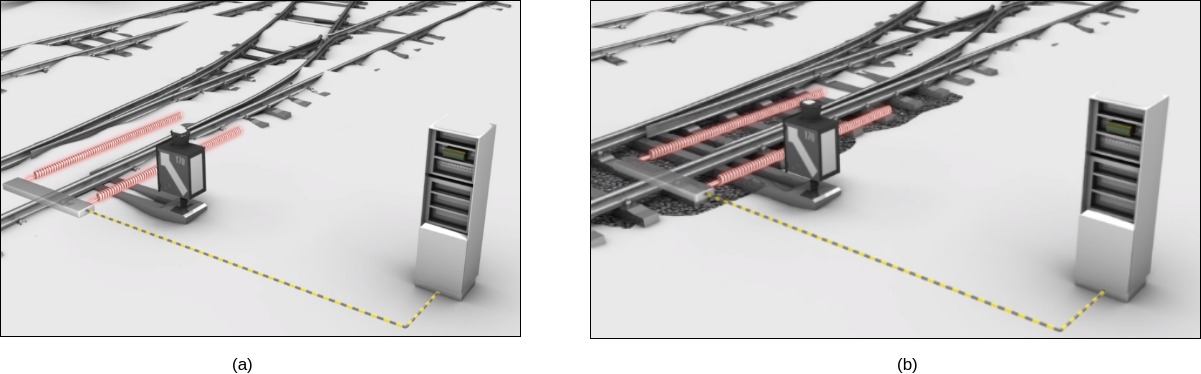
\includegraphics[width=17cm]{figures/requirements/railway_heater.jpg}
\caption[Pilz railway heater system]{Pilz railway heating system\cite{pilz_rail_engineering}}\label{pilz_railway_heater}
\end{figure}






\section{Requirement Analysis}

In this section, we present the functional and the non-functional requirements that our security layer should satisfy.

\subsection{Functional Requirements}

Based on DTLS, our security layer should provide the following requirements:

\renewcommand{\labelitemi}{$\bullet$}
\begin{itemize}
\item Authentication: Recipients of a message can identify their communication partners and can detect
if the sender information has been forged.\\

\item Integrity: Communication partners can detect changes to a message during transmission.\\

\item Confidentiality (Optional): If the messages are confidential, they could be encrypted and only
the authorized devices could be able to decrypt messages and read the content.
\end{itemize}

\subsection{Non-functional Requirements}

Our security layer should respect the following constraints:

\renewcommand{\labelitemi}{$\bullet$}
\begin{itemize}

\item Transparent integration: The security layer should not perform any changes to SafetyNETp application
layer state machine.\\

\item Easily Configurable: Changing the parameters of the security layer should be easy for SafeyNETp developers.\\

\item Time and memory constraints: The security layer needs to keep SafetyNETp cycle time as it is as much as possible
and to optimize memory consumption.\\

\item Maintainability: The security layer needs to be easy to understand and to maintain.


\end{itemize}

\section{Requirement Specification}

In this section, using a use case diagram, we formalize our requirements by illustrating the interaction between the security layer
and our only actor which consists of SafetyNETp application layer.

\begin{figure}[H]
\centering
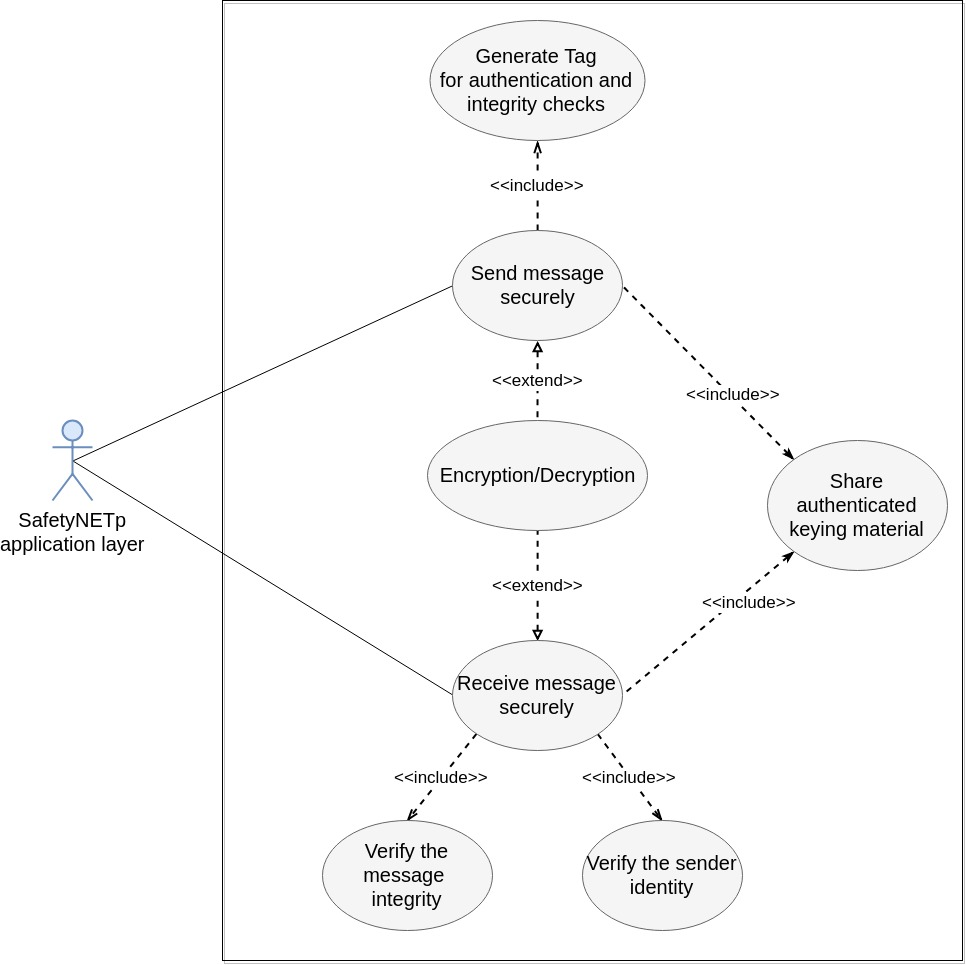
\includegraphics[width=13cm]{figures/requirements/use_case.jpg}
\caption{General use case diagram}\label{general_use_case_diagram}
\end{figure}

As depicted in \autoref{general_use_case_diagram}, our security layer allows SafetyNETp application layer to both, send and receive messages securely.
Indeed, we need first the establishment of shared authenticated keying material. Thereafter, if the operation
is sending, a tag will be generated by our security layer and sent to allow the receiver to authenticate the sender and verify the integrity of
the received message. If the operation is receiving, using the tag, the receiver is able to authenticate the sender and verify the message integrity.
In some application we may don't need confidentiality, therefore, the encryption is optional. In fact, in applications where
confidentiality is not required, sending data without encryption allows reducing significantly the CPU usage.

\section*{Conclusion}

After we set the requirements that our security layer should satisfy, we pass in the next chapter to discuss
the global and the detailed design.
